\scanpage{26}
Soit $X$ un ens. Une \uline{\unsure{décomposition|dècomposition|decomposition|disposition} binaire} de $X$ est un ens de deux parties de $X$
\[
(% BEGIN C026-S01
\unsure{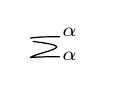
\begin{tikzpicture}[x=0.025em,y=-0.025em,baseline=(base),line cap=round,line join=round]
\coordinate (base) at (0,43);
\path[use as bounding box] (0,0) rectangle (84,56);
\begin{scope}[shift={(-602,-290)}]
\draw[line width=0.45pt] (606,305) .. controls (619.4,303) and (641,303) .. (648,303);
\draw[line width=0.45pt] (610,310) .. controls (618,311) and (645,314) .. (644,318) .. controls (642,323) and (613,328) .. (606,333) .. controls (622.8,332) and (639,332) .. (648,332);
\node[anchor=base west,inner sep=0pt,outer sep=0pt,font=\scriptsize] at (652,337) {$\alpha$};
\node[anchor=base west,inner sep=0pt,outer sep=0pt,font=\scriptsize] at (652,303) {$\alpha$};
\node[anchor=base west,inner sep=0pt,outer sep=0pt] at (602,333) {\phantom{$\Sigma_{\alpha}^{\alpha}$}};
\end{scope}
\end{tikzpicture}}
% END C026-S01
)_{\alpha\in\unsure{\mathcal E|\mathscr E|\varepsilon}}\qquad(\text{les ``hémisphères})
\]
dont la réunion est $X$, et dont \deleted{l'intersection} aucune n'est contenue dans l'autre -- on désigne par $E$ (``équateur'') l'intersection (on n'exclut pas qu'elle soit vide). Quand $X$ est un espace topologique, on \unsure{s'intéresse|s'intèresse|s'interesse} au cas où les % BEGIN C026-G01
\unsure{
\begin{tikzpicture}[x=0.025em,y=-0.025em,baseline=(base),line cap=round,line join=round]
\coordinate (base) at (0,49);
\path[use as bounding box] (0,0) rectangle (374,74);
\begin{scope}[shift={(-281,-857)}]
\draw[line width=0.45pt] (302,864) .. controls (320,865) and (317,883) .. (302,887) .. controls (294,896) and (300,908) .. (308,910) .. controls (315,909) and (316,900) .. (323,900) -- (333,905);
\draw[line width=0.55pt] (287,883) -- (331,883);
\draw[line width=0.45pt] (287,883) -- (312,895);
\node[anchor=base west,inner sep=0pt,outer sep=0pt] at (333,906) {émisphères};
\node[anchor=base west,inner sep=0pt,outer sep=0pt] at (282,906) {\phantom{\unsure{hémisphères|\deleted{h}émisphères}}};
\end{scope}
\end{tikzpicture}}
% END C026-G01
 $% BEGIN C026-S02
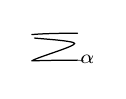
\begin{tikzpicture}[x=0.025em,y=-0.025em,baseline=(base),line cap=round,line join=round]
\coordinate (base) at (0,48);
\path[use as bounding box] (0,0) rectangle (101,62);
\begin{scope}[shift={(-765,-824)}]
\draw[line width=0.45pt] (771,834) .. controls (792.1,832) and (830,832) .. (837,832);
\draw[line width=0.45pt] (775,839) .. controls (783,840) and (834,843) .. (833,847) .. controls (831,852) and (778,867) .. (771,872) .. controls (797.4,871) and (828,871) .. (837,871);
\draw[line width=0.35pt,black!60] (837,871) -- (846,872);
\node[anchor=base west,inner sep=0pt,outer sep=0pt,font=\scriptsize] at (841,876) {$\alpha$};
\node[anchor=base west,inner sep=0pt,outer sep=0pt] at (765,872) {\phantom{$\Sigma_{\alpha}$}};
\end{scope}
\end{tikzpicture}
% END C026-S02
$ sont fermés, % BEGIN C026-G02
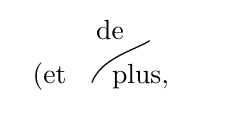
\begin{tikzpicture}[x=0.025em,y=-0.025em,baseline=(base),line cap=round,line join=round]
\coordinate (base) at (0,80);
\path[use as bounding box] (0,0) rectangle (268,119);
\begin{scope}[shift={(-1328,-776)}]
\node[anchor=base west,inner sep=0pt,outer sep=0pt] at (1335,857) {(et};
\node[anchor=base west,inner sep=0pt,outer sep=0pt] at (1427,793) {\inserted{de}};
\node[anchor=base west,inner sep=0pt,outer sep=0pt] at (1450,856) {plus,};
\draw[line width=0.45pt] (1421,855) .. controls (1434,820) and (1484,808) .. (1504,795);
\end{scope}
\end{tikzpicture}
% END C026-G02
 le plus souvent, % BEGIN C026-G03
\begin{tikzpicture}[x=0.025em,y=-0.025em,baseline=(base),line cap=round,line join=round]
\coordinate (base) at (0,109);
\path[use as bounding box] (0,0) rectangle (454,129);
\begin{scope}[shift={(-666,-875)}]
\node[anchor=base west,inner sep=0pt,outer sep=0pt] at (670,928) {\inserted{$% BEGIN C026-S03
\begin{tikzpicture}[x=0.025em,y=-0.025em,baseline=(base),line cap=round,line join=round]
\coordinate (base) at (0,41);
\path[use as bounding box] (0,0) rectangle (80,50);
\begin{scope}[shift={(-672,-892)}]
\draw[line width=0.45pt] (678,909) .. controls (691.4,907) and (713,907) .. (720,907);
\draw[line width=0.45pt] (678,909) .. controls (690,915) and (717,918) .. (716,922) .. controls (714,927) and (685,928) .. (678,933) .. controls (694.8,932) and (711,932) .. (720,932);
\node[anchor=base west,inner sep=0pt,outer sep=0pt,font=\scriptsize] at (724,937) {$\alpha$};
\node[anchor=base west,inner sep=0pt,outer sep=0pt,font=\scriptsize] at (724,907) {$\alpha$};
\node[anchor=base west,inner sep=0pt,outer sep=0pt] at (672,933) {\phantom{$\Sigma_{\alpha}^{\alpha}$}};
\end{scope}
\end{tikzpicture}
% END C026-S03
\ et\ % BEGIN C026-S04
\unsure{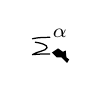
\begin{tikzpicture}[x=0.025em,y=-0.025em,baseline=(base),line cap=round,line join=round]
\coordinate (base) at (0,39);
\path[use as bounding box] (0,0) rectangle (66,53);
\begin{scope}[shift={(-824,-886)}]
\draw[line width=0.45pt] (831,902) .. controls (839.0,900) and (849,900) .. (856,900);
\draw[line width=0.45pt] (835,907) .. controls (843,908) and (853,911) .. (852,915) .. controls (850,920) and (838,920) .. (831,925) .. controls (841.0,924) and (847,924) .. (856,924);
\node[anchor=base west,inner sep=0pt,outer sep=0pt,font=\scriptsize] at (860,900) {$\alpha$};
\fill (859,922) -- (868,916) -- (875,921) -- (879,919) -- (880,929) -- (884,932) -- (881,937) -- (873,929) -- (866,929) -- cycle;
\node[anchor=base west,inner sep=0pt,outer sep=0pt] at (824,925) {\phantom{$\Sigma_{\deleted{\alpha}}^{\alpha}$}};
\end{scope}
\end{tikzpicture}}
% END C026-S04
\setminus E=% BEGIN C026-S05
\unsure{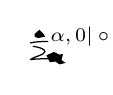
\begin{tikzpicture}[x=0.025em,y=-0.025em,baseline=(base),line cap=round,line join=round]
\coordinate (base) at (0,46);
\path[use as bounding box] (0,0) rectangle (82,56);
\begin{scope}[shift={(-959,-874)}]
\draw[line width=0.45pt] (963,896) .. controls (971.0,894) and (981,894) .. (988,894);
\draw[line width=0.45pt] (967,901) .. controls (975,902) and (985,905) .. (984,909) .. controls (982,914) and (970,915) .. (963,920) .. controls (973.0,919) and (979,919) .. (988,919);
\node[anchor=base west,inner sep=0pt,outer sep=0pt,font=\scriptsize] at (992,894) {$\alpha,\unsure{0|\circ|o}$};
\fill (986,914) -- (997,909) -- (1005,913) -- (1010,912) -- (1008,921) -- (1014,925) -- (1005,927) -- (999,923) -- (991,924) -- cycle;
\fill (969,883) -- (976,877) -- (982,883) -- (984,887) -- (974,889) -- (969,887) -- cycle;
\node[anchor=base west,inner sep=0pt,outer sep=0pt] at (959,920) {\phantom{$\Sigma_{\deleted{\alpha}}^{\deleted{\alpha}\alpha,0}$}};
\end{scope}
\end{tikzpicture}}
% END C026-S05
$}};
\node[anchor=base west,inner sep=0pt,outer sep=0pt] at (758,984) {connexes};
\node[anchor=base west,inner sep=0pt,outer sep=0pt] at (1050,984) {$% BEGIN C026-S06
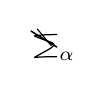
\begin{tikzpicture}[x=0.025em,y=-0.025em,baseline=(base),line cap=round,line join=round]
\coordinate (base) at (0,43);
\path[use as bounding box] (0,0) rectangle (69,55);
\begin{scope}[shift={(-1048,-936)}]
\draw[line width=0.45pt] (1058,948) .. controls (1068.2,946) and (1083,946) .. (1090,946);
\draw[line width=0.45pt] (1058,948) .. controls (1070,954) and (1087,957) .. (1086,961) .. controls (1084,966) and (1065,974) .. (1058,979) .. controls (1070.8,978) and (1081,978) .. (1090,978);
\node[anchor=base west,inner sep=0pt,outer sep=0pt,font=\scriptsize] at (1094,983) {$\alpha$};
\draw[line width=0.55pt] (1053,941) -- (1090,964);
\draw[line width=0.4pt] (1062,938) -- (1082,962);
\node[anchor=base west,inner sep=0pt,outer sep=0pt] at (1048,979) {\phantom{$\deleted{\Sigma_{\alpha}}$}};
\end{scope}
\end{tikzpicture}
% END C026-S06
$};
\draw[line width=0.4pt] (755,999) .. controls (737,969) and (747,950) .. (780,948) .. controls (846,948) and (922,949) .. (949,930) .. controls (954,926) and (956,922) .. (955,918);
\end{scope}
\end{tikzpicture}
% END C026-G03
 et où $E\ne\varnothing$); si les $% BEGIN C026-S07
\unsure{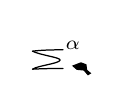
\begin{tikzpicture}[x=0.025em,y=-0.025em,baseline=(base),line cap=round,line join=round]
\coordinate (base) at (0,60);
\path[use as bounding box] (0,0) rectangle (101,71);
\begin{scope}[shift={(-785,-1001)}]
\draw[line width=0.45pt] (792,1035) .. controls (806.1,1033) and (829,1033) .. (836,1033);
\draw[line width=0.45pt] (792,1035) .. controls (804,1041) and (833,1044) .. (832,1048) .. controls (830,1053) and (799,1056) .. (792,1061) .. controls (809.6,1060) and (827,1060) .. (836,1060);
\node[anchor=base west,inner sep=0pt,outer sep=0pt,font=\scriptsize] at (840,1033) {$\alpha$};
\fill (849,1056) -- (862,1051) -- (870,1054) -- (871,1062) -- (877,1067) -- (872,1070) -- (866,1063) -- (856,1062) -- cycle;
\node[anchor=base west,inner sep=0pt,outer sep=0pt] at (785,1061) {\phantom{$\Sigma_{\deleted{\alpha}}^{\alpha}$}};
\end{scope}
\end{tikzpicture}}
% END C026-S07
$ connexes et $E% BEGIN C026-G04
\unsure{\begin{tikzpicture}[x=0.025em,y=-0.025em,baseline=(base),line cap=round,line join=round]
\coordinate (base) at (0,27);
\path[use as bounding box] (0,0) rectangle (39,36);
\begin{scope}[shift={(-1355,-1000)}]
\draw[line width=0.45pt] (1361,1018) -- (1385,1017);
\draw[line width=0.35pt] (1374,1010) .. controls (1382,1009) and (1386,1010) .. (1387,1012);
\draw[line width=0.45pt] (1379,1005) -- (1371,1031);
\node[anchor=base west,inner sep=0pt,outer sep=0pt] at (1360,1027) {\phantom{$\unsure{\ne|+}$}};
\end{scope}
\end{tikzpicture}}
% END C026-G04
\varnothing$, $X$ est connexe, si % BEGIN C026-G05
\begin{tikzpicture}[x=0.025em,y=-0.025em,baseline=(base),line cap=round,line join=round]
\coordinate (base) at (0,89);
\path[use as bounding box] (0,0) rectangle (540,106);
\begin{scope}[shift={(-600,-1068)}]
\node[anchor=base west,inner sep=0pt,outer sep=0pt] at (605,1101) {\inserted{$X$ connexe,}};
\node[anchor=base west,inner sep=0pt,outer sep=0pt] at (867,1084) {\rlap{et}\phantom{\inserted{\deleted{et}}}};
\draw[line width=0.55pt] (865,1080) -- (910,1080);
\node[anchor=base west,inner sep=0pt,outer sep=0pt] at (650,1157) {les};
\node[anchor=base west,inner sep=0pt,outer sep=0pt] at (770,1157) {$% BEGIN C026-S08
\begin{tikzpicture}[x=0.025em,y=-0.025em,baseline=(base),line cap=round,line join=round]
\coordinate (base) at (0,46);
\path[use as bounding box] (0,0) rectangle (112,60);
\begin{scope}[shift={(-767,-1106)}]
\draw[line width=0.45pt] (776,1125) .. controls (790.7,1123) and (815,1123) .. (822,1123);
\draw[line width=0.45pt] (776,1125) .. controls (788,1131) and (819,1134) .. (818,1138) .. controls (816,1143) and (783,1147) .. (776,1152) .. controls (794.4,1151) and (813,1151) .. (822,1151);
\node[anchor=base west,inner sep=0pt,outer sep=0pt,font=\scriptsize] at (826,1156) {$\alpha$};
\node[anchor=base west,inner sep=0pt,outer sep=0pt,font=\scriptsize] at (826,1123) {$\alpha,0$};
\node[anchor=base west,inner sep=0pt,outer sep=0pt] at (767,1152) {\phantom{$\Sigma_{\alpha}^{\alpha,0}$}};
\end{scope}
\end{tikzpicture}
% END C026-S08
$};
\node[anchor=base west,inner sep=0pt,outer sep=0pt] at (907,1140) {connexes};
\node[anchor=base west,inner sep=0pt,outer sep=0pt] at (1116,1141) {,};
\draw[line width=0.6pt] (643,1164) .. controls (784,1153) and (995,1132) .. (1106,1128);
\draw[line width=0.35pt,black!65] (643,1168) .. controls (628,1120) and (642,1120) .. (681,1114) .. controls (814,1087) and (929,1081) .. (965,1075) .. controls (974,1073) and (975,1078) .. (968,1080);
\node[anchor=base west,inner sep=0pt,outer sep=0pt] at (648,1157) {\phantom{\deleted{les $\Sigma_{\alpha}^{\alpha,0}$ connexes}}};
\end{scope}
\end{tikzpicture}
% END C026-G05
 on conclut \deleted{\unsure{aussitôt|aussitot}} que $% BEGIN C026-S09
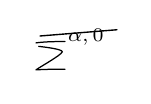
\begin{tikzpicture}[x=0.025em,y=-0.025em,baseline=(base),line cap=round,line join=round]
\coordinate (base) at (0,61);
\path[use as bounding box] (0,0) rectangle (138,69);
\begin{scope}[shift={(-472,-1227)}]
\draw[line width=0.45pt] (484,1249) .. controls (497.4,1247) and (519,1247) .. (526,1247);
\draw[line width=0.45pt] (488,1254) .. controls (496,1255) and (523,1258) .. (522,1262) .. controls (520,1267) and (491,1283) .. (484,1288) .. controls (500.8,1287) and (517,1287) .. (526,1287);
\node[anchor=base west,inner sep=0pt,outer sep=0pt,font=\scriptsize] at (530,1247) {$\alpha,0$};
\draw[line width=0.5pt] (490,1239) -- (601,1230);
\node[anchor=base west,inner sep=0pt,outer sep=0pt] at (472,1288) {\phantom{$\Sigma^{\alpha,0}$}};
\end{scope}
\end{tikzpicture}
% END C026-S09
\cap E\ne\varnothing$
% margin note written sideways
\reversemarginpar\margin{% BEGIN C026-G06
\diagram{\rotatebox{50}{\begin{tikzcd}[ampersand replacement=\&,column sep=2.8em,execute at end picture={
\begin{scope}[x=1mm,y=1mm,shift={(scLeft.center)}]
\node[anchor=base west,inner sep=0pt,outer sep=0pt] at (-2,8) {diagramme};
% The cancelled upper character has B primary, E and Sigma alternatives; paths occur once.
\node[anchor=base west,inner sep=0pt,outer sep=0pt] at (4,2) {\unsure{
\begin{tikzpicture}[x=0.12em,y=-0.12em,baseline=(base),line cap=round,line join=round]
\coordinate (base) at (0,7);\path[use as bounding box] (0,0) rectangle (8,8);
\draw[line width=0.5pt] (1,7) -- (1,1) -- (5,1) .. controls (8,1) and (8,3) .. (4,4) .. controls (9,4) and (8,7) .. (1,7);
\draw[line width=0.5pt] (0,2) -- (7,0) (0,6) -- (8,2) (0,8) -- (7,4);
\node[anchor=base west,inner sep=0pt,outer sep=0pt] at (0,7) {\phantom{$\deleted{B|E|\Sigma}$}};
\end{tikzpicture}}};
% One small point below the segment; no punctuation or algebraic role assigned.
\node[anchor=base west,inner sep=0pt,outer sep=0pt] at (3,-1.3) {\unsure{\begin{tikzpicture}[x=1mm,y=1mm,baseline=(base)]\coordinate (base) at (0,0);\path[use as bounding box] (0,0) rectangle (.7,.7);\fill (.3,.3) circle (.13);\end{tikzpicture}}};
\node[anchor=base west,inner sep=0pt,outer sep=0pt] at (-4,-6) {$% BEGIN C026-S15
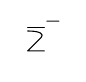
\begin{tikzpicture}[x=0.12em,y=-0.12em,baseline=(base),line cap=round,line join=round]
\coordinate (base) at (0,7);\path[use as bounding box] (0,0) rectangle (9,8);
\draw (0,0) -- (5,0);\draw (0,1) .. controls (4,1) and (5,2) .. (4,3) -- (0,7) -- (5,7);
\node[anchor=base west,inner sep=0pt,outer sep=0pt,font=\scriptsize] at (5,-.4) {$-$};
\end{tikzpicture}
% END C026-S15
\supset % BEGIN C026-E01
\unsure{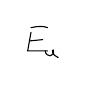
\begin{tikzpicture}[x=0.12em,y=-0.12em,baseline=(base),line cap=round,line join=round]
\coordinate (base) at (0,7);\path[use as bounding box] (0,0) rectangle (10,10);
\draw (1,0) .. controls (3,-.5) and (5,-.5) .. (6,0);
\draw (1,1.4) -- (0,7) -- (6,7);
\draw (.5,4) -- (4.5,3.6);
\draw (5.3,7) .. controls (5.4,9) and (8.3,9) .. (7.7,6.7) .. controls (7.2,6.6) and (7.3,8.3) .. (9.2,9);
\node[anchor=base west,inner sep=0pt,outer sep=0pt] at (0,7) {\phantom{$E_\alpha$}};
\end{tikzpicture}}
% END C026-E01
\subset% BEGIN C026-S16
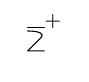
\begin{tikzpicture}[x=0.12em,y=-0.12em,baseline=(base),line cap=round,line join=round]
\coordinate (base) at (0,7);\path[use as bounding box] (0,0) rectangle (10,8);
\draw (0,0) -- (5,0);\draw (0,1) .. controls (4,1) and (5,2) .. (4,3) -- (0,7) -- (5,7);
\node[anchor=base west,inner sep=0pt,outer sep=0pt,font=\scriptsize] at (5,-.4) {$+$};
\end{tikzpicture}
% END C026-S16
$};
\end{scope}
}]
|[alias=scLeft]|\bullet\arrow[r,dash]\&\bullet
\end{tikzcd}}}
% END C026-G06
}\normalmarginpar%
(car $% BEGIN C026-S10
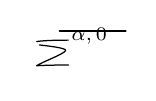
\begin{tikzpicture}[x=0.025em,y=-0.025em,baseline=(base),line cap=round,line join=round]
\coordinate (base) at (0,55);
\path[use as bounding box] (0,0) rectangle (145,66);
\begin{scope}[shift={(-1097,-1173)}]
\draw[line width=0.45pt] (1110,1193) .. controls (1124.7,1191) and (1149,1191) .. (1156,1191);
\draw[line width=0.45pt] (1114,1198) .. controls (1122,1199) and (1153,1202) .. (1152,1206) .. controls (1150,1211) and (1117,1223) .. (1110,1228) .. controls (1128.4,1227) and (1147,1227) .. (1156,1227);
\node[anchor=base west,inner sep=0pt,outer sep=0pt,font=\scriptsize] at (1160,1191) {$\alpha,0$};
\draw[line width=0.5pt] (1143,1178) -- (1239,1178);
\node[anchor=base west,inner sep=0pt,outer sep=0pt] at (1097,1228) {\phantom{$\Sigma^{\alpha,0}$}};
\end{scope}
\end{tikzpicture}
% END C026-S10
\cap E=% BEGIN C026-S11
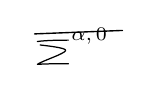
\begin{tikzpicture}[x=0.025em,y=-0.025em,baseline=(base),line cap=round,line join=round]
\coordinate (base) at (0,53);
\path[use as bounding box] (0,0) rectangle (141,62);
\begin{scope}[shift={(-1373,-1158)}]
\draw[line width=0.45pt] (1387,1178) .. controls (1401.4,1176) and (1425,1176) .. (1432,1176);
\draw[line width=0.45pt] (1391,1183) .. controls (1399,1184) and (1429,1187) .. (1428,1191) .. controls (1426,1196) and (1394,1206) .. (1387,1211) .. controls (1405.0,1210) and (1423,1210) .. (1432,1210);
\node[anchor=base west,inner sep=0pt,outer sep=0pt,font=\scriptsize] at (1436,1176) {$\alpha,0$};
\draw[line width=0.5pt] (1383,1167) -- (1510,1162);
\node[anchor=base west,inner sep=0pt,outer sep=0pt] at (1373,1211) {\phantom{$\Sigma^{\alpha,0}$}};
\end{scope}
\end{tikzpicture}
% END C026-S11
\setminus% BEGIN C026-S12
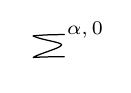
\begin{tikzpicture}[x=0.025em,y=-0.025em,baseline=(base),line cap=round,line join=round]
\coordinate (base) at (0,43);
\path[use as bounding box] (0,0) rectangle (109,53);
\begin{scope}[shift={(-1535,-1171)}]
\draw[line width=0.45pt] (1543,1183) .. controls (1557.4,1181) and (1581,1181) .. (1588,1181);
\draw[line width=0.45pt] (1543,1183) .. controls (1555,1189) and (1585,1192) .. (1584,1196) .. controls (1582,1201) and (1550,1209) .. (1543,1214) .. controls (1561.0,1213) and (1579,1213) .. (1588,1213);
\node[anchor=base west,inner sep=0pt,outer sep=0pt,font=\scriptsize] at (1592,1181) {$\alpha,0$};
\node[anchor=base west,inner sep=0pt,outer sep=0pt] at (1535,1214) {\phantom{$\Sigma^{\alpha,0}$}};
\end{scope}
\end{tikzpicture}
% END C026-S12
$, et $% BEGIN C026-S13
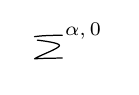
\begin{tikzpicture}[x=0.025em,y=-0.025em,baseline=(base),line cap=round,line join=round]
\coordinate (base) at (0,45);
\path[use as bounding box] (0,0) rectangle (120,56);
\begin{scope}[shift={(-408,-1367)}]
\draw[line width=0.45pt] (418,1380) .. controls (430.8,1378) and (451,1378) .. (458,1378);
\draw[line width=0.45pt] (422,1385) .. controls (430,1386) and (455,1389) .. (454,1393) .. controls (452,1398) and (425,1407) .. (418,1412) .. controls (434.0,1411) and (449,1411) .. (458,1411);
\node[anchor=base west,inner sep=0pt,outer sep=0pt,font=\scriptsize] at (462,1378) {$\alpha,0$};
\node[anchor=base west,inner sep=0pt,outer sep=0pt] at (408,1412) {\phantom{$\Sigma^{\alpha,0}$}};
\end{scope}
\end{tikzpicture}
% END C026-S13
$ ne peut \unsure{être|etre} \unsure{à|:} la fois ouvert et fermé car $% BEGIN C026-S14
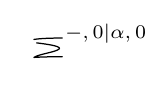
\begin{tikzpicture}[x=0.025em,y=-0.025em,baseline=(base),line cap=round,line join=round]
\coordinate (base) at (0,43);
\path[use as bounding box] (0,0) rectangle (129,56);
\begin{scope}[shift={(-451,-1471)}]
\draw[line width=0.45pt] (460,1488) .. controls (473.1,1486) and (494,1486) .. (501,1486);
\draw[line width=0.45pt] (464,1493) .. controls (472,1494) and (498,1497) .. (497,1501) .. controls (495,1506) and (467,1509) .. (460,1514) .. controls (476.4,1513) and (492,1513) .. (501,1513);
\node[anchor=base west,inner sep=0pt,outer sep=0pt,font=\scriptsize] at (505,1486) {$\unsure{-,0|\alpha,0|-\alpha,0}$};
\node[anchor=base west,inner sep=0pt,outer sep=0pt] at (451,1514) {\phantom{$\Sigma^{\unsure{-,0|\alpha,0|-\alpha,0}}$}};
\end{scope}
\end{tikzpicture}
% END C026-S14
$, est $\underset{\text{% BEGIN C026-M02
\unsure{\begin{tikzpicture}[x=0.025em,y=-0.025em,baseline=(base),line cap=round,line join=round]
\coordinate (base) at (0,13);
\path[use as bounding box] (0,0) rectangle (24,17);
\begin{scope}[shift={(-731,-1520)}]
\draw[line width=0.35pt] (734,1523) -- (737,1526);
\fill[black!60] (742,1528) circle (.65);
\fill[black!45] (747,1530) circle (.6);
\fill[black!35] (752,1532) circle (.5);
\end{scope}
\end{tikzpicture}}
% END C026-M02
}}{\text{un}}$ ouvert $\ne\varnothing$ et $\ne X$)

Considérons deux décompositions binaires % BEGIN C026-G08
\begin{tikzpicture}[x=0.025em,y=-0.025em,baseline=(base),line cap=round,line join=round]
\coordinate (base) at (0,69);
\path[use as bounding box] (0,0) rectangle (610,122);
\begin{scope}[shift={(-100,-1630)}]
\node[anchor=base west,inner sep=0pt,outer sep=0pt] at (107,1699) {$\{% BEGIN C026-S17
\begin{tikzpicture}[x=0.025em,y=-0.025em,baseline=(base),line cap=round,line join=round]
\coordinate (base) at (0,53);
\path[use as bounding box] (0,0) rectangle (65,64);
\begin{scope}[shift={(-115,-1651)}]
\draw[line width=0.45pt] (122,1667) .. controls (133.8,1665) and (152,1665) .. (159,1665);
\draw[line width=0.45pt] (122,1667) .. controls (134,1673) and (156,1676) .. (155,1680) .. controls (153,1685) and (129,1699) .. (122,1704) .. controls (136.8,1703) and (150,1703) .. (159,1703);
\draw[line width=0.35pt] (124,1674) -- (146,1679) -- (128,1683);
\node[anchor=base west,inner sep=0pt,outer sep=0pt,font=\scriptsize] at (163,1708) {$1$};
\node[anchor=base west,inner sep=0pt,outer sep=0pt,font=\scriptsize] at (163,1665) {$+$};
\node[anchor=base west,inner sep=0pt,outer sep=0pt] at (115,1704) {\phantom{$\Sigma_{1}^{+}$}};
\end{scope}
\end{tikzpicture}
% END C026-S17
,% BEGIN C026-S18
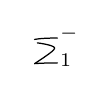
\begin{tikzpicture}[x=0.025em,y=-0.025em,baseline=(base),line cap=round,line join=round]
\coordinate (base) at (0,52);
\path[use as bounding box] (0,0) rectangle (63,62);
\begin{scope}[shift={(-190,-1648)}]
\draw[line width=0.45pt] (200,1665) .. controls (210.6,1663) and (226,1663) .. (233,1663);
\draw[line width=0.45pt] (204,1670) .. controls (212,1671) and (230,1674) .. (229,1678) .. controls (227,1683) and (207,1695) .. (200,1700) .. controls (213.2,1699) and (224,1699) .. (233,1699);
\node[anchor=base west,inner sep=0pt,outer sep=0pt,font=\scriptsize] at (237,1704) {$1$};
\node[anchor=base west,inner sep=0pt,outer sep=0pt,font=\scriptsize] at (237,1663) {$-$};
\node[anchor=base west,inner sep=0pt,outer sep=0pt] at (190,1700) {\phantom{$\Sigma_{1}^{-}$}};
\end{scope}
\end{tikzpicture}
% END C026-S18
\},\unsure{[|(}% BEGIN C026-S19
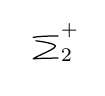
\begin{tikzpicture}[x=0.025em,y=-0.025em,baseline=(base),line cap=round,line join=round]
\coordinate (base) at (0,45);
\path[use as bounding box] (0,0) rectangle (71,58);
\begin{scope}[shift={(-330,-1636)}]
\draw[line width=0.45pt] (338,1650) .. controls (349.5,1648) and (367,1648) .. (374,1648);
\draw[line width=0.45pt] (342,1655) .. controls (350,1656) and (371,1659) .. (370,1663) .. controls (368,1668) and (345,1676) .. (338,1681) .. controls (352.4,1680) and (365,1680) .. (374,1680);
\node[anchor=base west,inner sep=0pt,outer sep=0pt,font=\scriptsize] at (378,1685) {$2$};
\node[anchor=base west,inner sep=0pt,outer sep=0pt,font=\scriptsize] at (378,1648) {$+$};
\node[anchor=base west,inner sep=0pt,outer sep=0pt] at (330,1681) {\phantom{$\Sigma_{2}^{+}$}};
\end{scope}
\end{tikzpicture}
% END C026-S19
,% BEGIN C026-S20
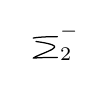
\begin{tikzpicture}[x=0.025em,y=-0.025em,baseline=(base),line cap=round,line join=round]
\coordinate (base) at (0,44);
\path[use as bounding box] (0,0) rectangle (61,55);
\begin{scope}[shift={(-407,-1634)}]
\draw[line width=0.45pt] (415,1649) .. controls (426.2,1647) and (443,1647) .. (450,1647);
\draw[line width=0.45pt] (419,1654) .. controls (427,1655) and (447,1658) .. (446,1662) .. controls (444,1667) and (422,1673) .. (415,1678) .. controls (429.0,1677) and (441,1677) .. (450,1677);
\node[anchor=base west,inner sep=0pt,outer sep=0pt,font=\scriptsize] at (454,1682) {$2$};
\node[anchor=base west,inner sep=0pt,outer sep=0pt,font=\scriptsize] at (454,1647) {$-$};
\node[anchor=base west,inner sep=0pt,outer sep=0pt] at (407,1678) {\phantom{$\Sigma_{2}^{-}$}};
\end{scope}
\end{tikzpicture}
% END C026-S20
\}$};
\node[anchor=base west,inner sep=0pt,outer sep=0pt] at (518,1669) {\rlap{distinctes}\phantom{\deleted{distinctes}}};
\draw[line width=0.45pt] (512,1681) -- (561,1644) -- (540,1679) -- (604,1640) -- (584,1671) -- (648,1635);
\draw[line width=0.45pt] (518,1680) -- (698,1657);
\node[anchor=base west,inner sep=0pt,outer sep=0pt] at (272,1730) {\inserted{de $X$,}};
\draw[line width=0.4pt] (229,1744) .. controls (240,1700) and (328,1709) .. (401,1708) .. controls (466,1702) and (523,1692) .. (545,1688) .. controls (562,1696) and (584,1692) .. (594,1690);
\end{scope}
\end{tikzpicture}
% END C026-G08
 on dit qu'elles sont % BEGIN C026-G07
\begin{tikzpicture}[x=0.025em,y=-0.025em,baseline=(base),line cap=round,line join=round]
\coordinate (base) at (0,38);
\path[use as bounding box] (0,0) rectangle (453,84);
\begin{scope}[shift={(-1180,-1620)}]
\node[anchor=base west,inner sep=0pt,outer sep=0pt] at (1188,1658) {non \unsure{panachées|penchées|parallèles}};
\draw[line width=0.45pt] (1228,1685) -- (1622,1668);
\node[anchor=base west,inner sep=0pt,outer sep=0pt] at (1188,1658) {\phantom{\uline{non panachées}}};
\node[anchor=base west,inner sep=0pt,outer sep=0pt] at (1581,1694) {\unsure{\begin{tikzpicture}[x=0.025em,y=-0.025em,baseline=(base)]\coordinate (base) at (0,10);\path[use as bounding box] (0,0) rectangle (12,16);\fill (7,4) circle (1.15);\fill (3,11) circle (1.05);\end{tikzpicture}}};
\end{scope}
\end{tikzpicture}
% END C026-G07
 % BEGIN C026-G09
\begin{tikzpicture}[x=0.025em,y=-0.025em,baseline=(base),line cap=round,line join=round]
\coordinate (base) at (0,121);
\path[use as bounding box] (0,0) rectangle (659,142);
\begin{scope}[shift={(-280,-1716)}]
\node[anchor=base west,inner sep=0pt,outer sep=0pt] at (286,1852) {si};
\node[anchor=base west,inner sep=0pt,outer sep=0pt] at (370,1774) {\inserted{elles sont \uline{distinctes}, et si}};
\node[anchor=base west,inner sep=0pt,outer sep=0pt] at (386,1837) {% BEGIN C026-G09a
\unsure{\begin{tikzpicture}[x=0.025em,y=-0.025em,baseline=(base),line cap=round,line join=round]
\coordinate (base) at (0,13);
\path[use as bounding box] (0,0) rectangle (76,20);
\begin{scope}[shift={(-384,-1824)}]
\draw[line width=0.4pt] (389,1835) -- (391,1831);
\draw[line width=0.35pt,black!55] (402,1834) .. controls (413,1832) and (424,1830) .. (433,1831);
\draw[line width=0.35pt,black!60] (445,1831) .. controls (450,1830) and (453,1832) .. (455,1833);
\node[anchor=base west,inner sep=0pt,outer sep=0pt] at (386,1836) {\phantom{\unsure{on}}};
\end{scope}
\end{tikzpicture}}
% END C026-G09a
};
\node[anchor=base west,inner sep=0pt,outer sep=0pt] at (510,1816) {peut trouver};
\draw[line width=0.4pt] (373,1850) .. controls (361,1817) and (378,1804) .. (415,1800) .. controls (563,1777) and (766,1759) .. (925,1737) .. controls (932,1736) and (932,1731) .. (928,1728);
\end{scope}
\end{tikzpicture}
% END C026-G09
 $% BEGIN C026-S21
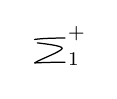
\begin{tikzpicture}[x=0.025em,y=-0.025em,baseline=(base),line cap=round,line join=round]
\coordinate (base) at (0,51);
\path[use as bounding box] (0,0) rectangle (89,62);
\begin{scope}[shift={(-927,-1744)}]
\draw[line width=0.45pt] (937,1761) .. controls (951.1,1759) and (974,1759) .. (981,1759);
\draw[line width=0.45pt] (941,1766) .. controls (949,1767) and (978,1770) .. (977,1774) .. controls (975,1779) and (944,1790) .. (937,1795) .. controls (954.6,1794) and (972,1794) .. (981,1794);
\node[anchor=base west,inner sep=0pt,outer sep=0pt,font=\scriptsize] at (985,1799) {$1$};
\node[anchor=base west,inner sep=0pt,outer sep=0pt,font=\scriptsize] at (985,1759) {$+$};
\node[anchor=base west,inner sep=0pt,outer sep=0pt] at (927,1795) {\phantom{$\Sigma_{1}^{+}$}};
\end{scope}
\end{tikzpicture}
% END C026-S21
$ dans l'une, $% BEGIN C026-S22
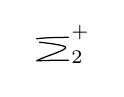
\begin{tikzpicture}[x=0.025em,y=-0.025em,baseline=(base),line cap=round,line join=round]
\coordinate (base) at (0,48);
\path[use as bounding box] (0,0) rectangle (98,60);
\begin{scope}[shift={(-1412,-1720)}]
\draw[line width=0.45pt] (1425,1736) .. controls (1439.7,1734) and (1464,1734) .. (1471,1734);
\draw[line width=0.45pt] (1429,1741) .. controls (1437,1742) and (1468,1745) .. (1467,1749) .. controls (1465,1754) and (1432,1763) .. (1425,1768) .. controls (1443.4,1767) and (1462,1767) .. (1471,1767);
\node[anchor=base west,inner sep=0pt,outer sep=0pt,font=\scriptsize] at (1475,1772) {$2$};
\node[anchor=base west,inner sep=0pt,outer sep=0pt,font=\scriptsize] at (1475,1734) {$+$};
\node[anchor=base west,inner sep=0pt,outer sep=0pt] at (1412,1768) {\phantom{$\Sigma_{2}^{+}$}};
\end{scope}
\end{tikzpicture}
% END C026-S22
$ dans l'autre, tels que
\[
% BEGIN C026-S23
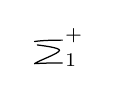
\begin{tikzpicture}[x=0.025em,y=-0.025em,baseline=(base),line cap=round,line join=round]
\coordinate (base) at (0,52);
\path[use as bounding box] (0,0) rectangle (97,64);
\begin{scope}[shift={(-648,-1947)}]
\draw[line width=0.45pt] (658,1967) .. controls (670.8,1965) and (691,1965) .. (698,1965);
\draw[line width=0.45pt] (662,1972) .. controls (670,1973) and (695,1976) .. (694,1980) .. controls (692,1985) and (665,1994) .. (658,1999) .. controls (674.0,1998) and (689,1998) .. (698,1998);
\node[anchor=base west,inner sep=0pt,outer sep=0pt,font=\scriptsize] at (702,2003) {$1$};
\node[anchor=base west,inner sep=0pt,outer sep=0pt,font=\scriptsize] at (702,1965) {$+$};
\node[anchor=base west,inner sep=0pt,outer sep=0pt] at (648,1999) {\phantom{$\Sigma_{1}^{+}$}};
\end{scope}
\end{tikzpicture}
% END C026-S23
\cap% BEGIN C026-S24
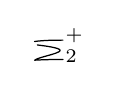
\begin{tikzpicture}[x=0.025em,y=-0.025em,baseline=(base),line cap=round,line join=round]
\coordinate (base) at (0,47);
\path[use as bounding box] (0,0) rectangle (102,60);
\begin{scope}[shift={(-804,-1947)}]
\draw[line width=0.45pt] (814,1967) .. controls (827.1,1965) and (848,1965) .. (855,1965);
\draw[line width=0.45pt] (818,1972) .. controls (826,1973) and (852,1976) .. (851,1980) .. controls (849,1985) and (821,1989) .. (814,1994) .. controls (830.4,1993) and (846,1993) .. (855,1993);
\node[anchor=base west,inner sep=0pt,outer sep=0pt,font=\scriptsize] at (859,1998) {$2$};
\node[anchor=base west,inner sep=0pt,outer sep=0pt,font=\scriptsize] at (859,1965) {$+$};
\node[anchor=base west,inner sep=0pt,outer sep=0pt] at (804,1994) {\phantom{$\Sigma_{2}^{+}$}};
\end{scope}
\end{tikzpicture}
% END C026-S24
=\varnothing\qquad(\text{d’où }E_1\cap E_2=\varnothing)
\]
on a alors
\[
\begin{aligned}
% BEGIN C026-S25
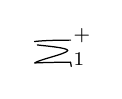
\begin{tikzpicture}[x=0.025em,y=-0.025em,baseline=(base),line cap=round,line join=round]
\coordinate (base) at (0,51);
\path[use as bounding box] (0,0) rectangle (95,63);
\begin{scope}[shift={(-648,-2097)}]
\draw[line width=0.45pt] (658,2117) .. controls (674.6,2115) and (703,2115) .. (710,2115);
\draw[line width=0.45pt] (662,2122) .. controls (670,2123) and (707,2126) .. (706,2130) .. controls (704,2135) and (665,2143) .. (658,2148) .. controls (678.8,2147) and (701,2147) .. (710,2147);
\draw[line width=0.45pt] (710,2147) -- (711,2153);
\node[anchor=base west,inner sep=0pt,outer sep=0pt,font=\scriptsize] at (714,2152) {$1$};
\node[anchor=base west,inner sep=0pt,outer sep=0pt,font=\scriptsize] at (714,2115) {$+$};
\node[anchor=base west,inner sep=0pt,outer sep=0pt] at (648,2148) {\phantom{$\Sigma_{1}^{+}$}};
\end{scope}
\end{tikzpicture}
% END C026-S25
&% BEGIN C026-G10
\unsure{
\begin{tikzpicture}[x=0.025em,y=-0.025em,baseline=(base),line cap=round,line join=round]
\coordinate (base) at (0,37);
\path[use as bounding box] (0,0) rectangle (49,46);
\begin{scope}[shift={(-748,-2100)}]
\draw[line width=0.55pt] (786,2108) .. controls (770,2103) and (758,2114) .. (761,2127) .. controls (765,2138) and (780,2135) .. (790,2135);
\draw[line width=0.4pt] (755,2141) .. controls (757,2129) and (764,2120) .. (769,2123) -- (779,2135);
\node[anchor=base west,inner sep=0pt,outer sep=0pt] at (753,2135) {\phantom{$\unsure{\deleted{\cap}\subset|\subset|\in}$}};
\end{scope}
\end{tikzpicture}}
% END C026-G10
% BEGIN C026-S26
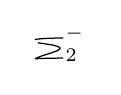
\begin{tikzpicture}[x=0.025em,y=-0.025em,baseline=(base),line cap=round,line join=round]
\coordinate (base) at (0,45);
\path[use as bounding box] (0,0) rectangle (94,56);
\begin{scope}[shift={(-790,-2089)}]
\draw[line width=0.45pt] (801,2106) .. controls (813.8,2104) and (834,2104) .. (841,2104);
\draw[line width=0.45pt] (805,2111) .. controls (813,2112) and (838,2115) .. (837,2119) .. controls (835,2124) and (808,2129) .. (801,2134) .. controls (817.0,2133) and (832,2133) .. (841,2133);
\node[anchor=base west,inner sep=0pt,outer sep=0pt,font=\scriptsize] at (845,2138) {$2$};
\node[anchor=base west,inner sep=0pt,outer sep=0pt,font=\scriptsize] at (845,2104) {$-$};
\node[anchor=base west,inner sep=0pt,outer sep=0pt] at (790,2134) {\phantom{$\Sigma_{2}^{-}$}};
\end{scope}
\end{tikzpicture}
% END C026-S26
\ % BEGIN C026-G11

\begin{tikzpicture}[x=0.025em,y=-0.025em,baseline=(base),line cap=round,line join=round]
\coordinate (base) at (0,40);
\path[use as bounding box] (0,0) rectangle (88,57);
\begin{scope}[shift={(-899,-2093)}]
\node[anchor=base west,inner sep=0pt,outer sep=0pt] at (906,2133) {\rlap{$\ne\varnothing$}\phantom{\deleted{$\ne\varnothing$}}};
\draw[line width=0.65pt] (903,2117) -- (947,2114) (904,2128) -- (959,2112) (911,2137) -- (952,2104) (948,2147) -- (981,2098);
\end{scope}
\end{tikzpicture}
% END C026-G11
\quad\text{i.e.}\quad% BEGIN C026-S27
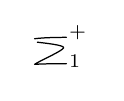
\begin{tikzpicture}[x=0.025em,y=-0.025em,baseline=(base),line cap=round,line join=round]
\coordinate (base) at (0,53);
\path[use as bounding box] (0,0) rectangle (98,65);
\begin{scope}[shift={(-1132,-2074)}]
\draw[line width=0.45pt] (1142,2090) .. controls (1156.7,2088) and (1181,2088) .. (1188,2088);
\draw[line width=0.45pt] (1146,2095) .. controls (1154,2096) and (1185,2099) .. (1184,2103) .. controls (1182,2108) and (1149,2122) .. (1142,2127) .. controls (1160.4,2126) and (1179,2126) .. (1188,2126);
\node[anchor=base west,inner sep=0pt,outer sep=0pt,font=\scriptsize] at (1192,2131) {$1$};
\node[anchor=base west,inner sep=0pt,outer sep=0pt,font=\scriptsize] at (1192,2088) {$+$};
\node[anchor=base west,inner sep=0pt,outer sep=0pt] at (1132,2127) {\phantom{$\Sigma_{1}^{+}$}};
\end{scope}
\end{tikzpicture}
% END C026-S27
\cap% BEGIN C026-S28
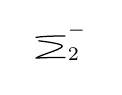
\begin{tikzpicture}[x=0.025em,y=-0.025em,baseline=(base),line cap=round,line join=round]
\coordinate (base) at (0,44);
\path[use as bounding box] (0,0) rectangle (96,57);
\begin{scope}[shift={(-1252,-2076)}]
\draw[line width=0.45pt] (1264,2090) .. controls (1277.4,2088) and (1299,2088) .. (1306,2088);
\draw[line width=0.45pt] (1268,2095) .. controls (1276,2096) and (1303,2099) .. (1302,2103) .. controls (1300,2108) and (1271,2115) .. (1264,2120) .. controls (1280.8,2119) and (1297,2119) .. (1306,2119);
\node[anchor=base west,inner sep=0pt,outer sep=0pt,font=\scriptsize] at (1310,2124) {$2$};
\node[anchor=base west,inner sep=0pt,outer sep=0pt,font=\scriptsize] at (1310,2088) {$-$};
\node[anchor=base west,inner sep=0pt,outer sep=0pt] at (1252,2120) {\phantom{$\Sigma_{2}^{-}$}};
\end{scope}
\end{tikzpicture}
% END C026-S28
=% BEGIN C026-S29
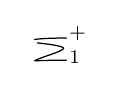
\begin{tikzpicture}[x=0.025em,y=-0.025em,baseline=(base),line cap=round,line join=round]
\coordinate (base) at (0,48);
\path[use as bounding box] (0,0) rectangle (95,60);
\begin{scope}[shift={(-1395,-2067)}]
\draw[line width=0.45pt] (1405,2084) .. controls (1419.7,2082) and (1444,2082) .. (1451,2082);
\draw[line width=0.45pt] (1409,2089) .. controls (1417,2090) and (1448,2093) .. (1447,2097) .. controls (1445,2102) and (1412,2110) .. (1405,2115) .. controls (1423.4,2114) and (1442,2114) .. (1451,2114);
\node[anchor=base west,inner sep=0pt,outer sep=0pt,font=\scriptsize] at (1455,2119) {$1$};
\node[anchor=base west,inner sep=0pt,outer sep=0pt,font=\scriptsize] at (1455,2082) {$+$};
\node[anchor=base west,inner sep=0pt,outer sep=0pt] at (1395,2115) {\phantom{$\Sigma_{1}^{+}$}};
\end{scope}
\end{tikzpicture}
% END C026-S29
\\
% BEGIN C026-S30
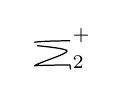
\begin{tikzpicture}[x=0.025em,y=-0.025em,baseline=(base),line cap=round,line join=round]
\coordinate (base) at (0,55);
\path[use as bounding box] (0,0) rectangle (106,68);
\begin{scope}[shift={(-644,-2177)}]
\draw[line width=0.45pt] (654,2198) .. controls (670.3,2196) and (698,2196) .. (705,2196);
\draw[line width=0.45pt] (658,2203) .. controls (666,2204) and (702,2207) .. (701,2211) .. controls (699,2216) and (661,2227) .. (654,2232) .. controls (674.4,2231) and (696,2231) .. (705,2231);
\draw[line width=0.45pt] (705,2231) -- (706,2237);
\node[anchor=base west,inner sep=0pt,outer sep=0pt,font=\scriptsize] at (709,2236) {$2$};
\node[anchor=base west,inner sep=0pt,outer sep=0pt,font=\scriptsize] at (709,2196) {$+$};
\node[anchor=base west,inner sep=0pt,outer sep=0pt] at (644,2232) {\phantom{$\Sigma_{2}^{+}$}};
\end{scope}
\end{tikzpicture}
% END C026-S30
&\subset% BEGIN C026-S31
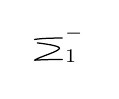
\begin{tikzpicture}[x=0.025em,y=-0.025em,baseline=(base),line cap=round,line join=round]
\coordinate (base) at (0,47);
\path[use as bounding box] (0,0) rectangle (91,63);
\begin{scope}[shift={(-805,-2178)}]
\draw[line width=0.45pt] (815,2195) .. controls (827.8,2193) and (848,2193) .. (855,2193);
\draw[line width=0.45pt] (819,2200) .. controls (827,2201) and (852,2204) .. (851,2208) .. controls (849,2213) and (822,2220) .. (815,2225) .. controls (831.0,2224) and (846,2224) .. (855,2224);
\node[anchor=base west,inner sep=0pt,outer sep=0pt,font=\scriptsize] at (859,2229) {$1$};
\node[anchor=base west,inner sep=0pt,outer sep=0pt,font=\scriptsize] at (859,2193) {$-$};
\node[anchor=base west,inner sep=0pt,outer sep=0pt] at (805,2225) {\phantom{$\Sigma_{1}^{-}$}};
\end{scope}
\end{tikzpicture}
% END C026-S31
\qquad\qquad\text{\unsure{i.e|i.e.|ie}}\quad% BEGIN C026-S32
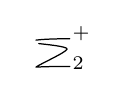
\begin{tikzpicture}[x=0.025em,y=-0.025em,baseline=(base),line cap=round,line join=round]
\coordinate (base) at (0,57);
\path[use as bounding box] (0,0) rectangle (103,70);
\begin{scope}[shift={(-1135,-2165)}]
\draw[line width=0.45pt] (1147,2183) .. controls (1162.7,2181) and (1189,2181) .. (1196,2181);
\draw[line width=0.45pt] (1151,2188) .. controls (1159,2189) and (1193,2192) .. (1192,2196) .. controls (1190,2201) and (1154,2217) .. (1147,2222) .. controls (1166.6,2221) and (1187,2221) .. (1196,2221);
\node[anchor=base west,inner sep=0pt,outer sep=0pt,font=\scriptsize] at (1200,2226) {$2$};
\node[anchor=base west,inner sep=0pt,outer sep=0pt,font=\scriptsize] at (1200,2181) {$+$};
\node[anchor=base west,inner sep=0pt,outer sep=0pt] at (1135,2222) {\phantom{$\Sigma_{2}^{+}$}};
\end{scope}
\end{tikzpicture}
% END C026-S32
\cap% BEGIN C026-S33
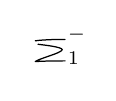
\begin{tikzpicture}[x=0.025em,y=-0.025em,baseline=(base),line cap=round,line join=round]
\coordinate (base) at (0,49);
\path[use as bounding box] (0,0) rectangle (87,66);
\begin{scope}[shift={(-1268,-2169)}]
\draw[line width=0.45pt] (1279,2188) .. controls (1292.8,2186) and (1315,2186) .. (1322,2186);
\draw[line width=0.45pt] (1283,2193) .. controls (1291,2194) and (1319,2197) .. (1318,2201) .. controls (1316,2206) and (1286,2213) .. (1279,2218) .. controls (1296.2,2217) and (1313,2217) .. (1322,2217);
\node[anchor=base west,inner sep=0pt,outer sep=0pt,font=\scriptsize] at (1326,2222) {$1$};
\node[anchor=base west,inner sep=0pt,outer sep=0pt,font=\scriptsize] at (1326,2186) {$-$};
\node[anchor=base west,inner sep=0pt,outer sep=0pt] at (1268,2218) {\phantom{$\Sigma_{1}^{-}$}};
\end{scope}
\end{tikzpicture}
% END C026-S33
=% BEGIN C026-S34
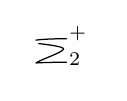
\begin{tikzpicture}[x=0.025em,y=-0.025em,baseline=(base),line cap=round,line join=round]
\coordinate (base) at (0,51);
\path[use as bounding box] (0,0) rectangle (103,65);
\begin{scope}[shift={(-1374,-2164)}]
\draw[line width=0.45pt] (1386,2182) .. controls (1400.1,2180) and (1423,2180) .. (1430,2180);
\draw[line width=0.45pt] (1390,2187) .. controls (1398,2188) and (1427,2191) .. (1426,2195) .. controls (1424,2200) and (1393,2210) .. (1386,2215) .. controls (1403.6,2214) and (1421,2214) .. (1430,2214);
\node[anchor=base west,inner sep=0pt,outer sep=0pt,font=\scriptsize] at (1434,2219) {$2$};
\node[anchor=base west,inner sep=0pt,outer sep=0pt,font=\scriptsize] at (1434,2180) {$+$};
\node[anchor=base west,inner sep=0pt,outer sep=0pt] at (1374,2215) {\phantom{$\Sigma_{2}^{+}$}};
\end{scope}
\end{tikzpicture}
% END C026-S34
\\
% BEGIN C026-S35
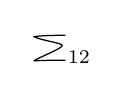
\begin{tikzpicture}[x=0.025em,y=-0.025em,baseline=(base),line cap=round,line join=round]
\coordinate (base) at (0,48);
\path[use as bounding box] (0,0) rectangle (96,62);
\begin{scope}[shift={(-529,-2270)}]
\draw[line width=0.45pt] (538,2283) .. controls (552.4,2281) and (576,2281) .. (583,2281);
\draw[line width=0.45pt] (538,2283) .. controls (550,2289) and (580,2292) .. (579,2296) .. controls (577,2301) and (545,2313) .. (538,2318) .. controls (556.0,2317) and (574,2317) .. (583,2317);
\node[anchor=base west,inner sep=0pt,outer sep=0pt,font=\scriptsize] at (587,2322) {$12$};
\node[anchor=base west,inner sep=0pt,outer sep=0pt] at (529,2318) {\phantom{$\Sigma_{12}$}};
\end{scope}
\end{tikzpicture}
% END C026-S35
&% BEGIN C026-G12
\unsure{\begin{tikzpicture}[x=0.025em,y=-0.025em,baseline=(base),line cap=round,line join=round]
\coordinate (base) at (0,57);
\path[use as bounding box] (0,0) rectangle (43,62);
\begin{scope}[shift={(-610,-2250)}]
\node[anchor=base west,inner sep=0pt,outer sep=0pt,font=\scriptsize] at (613,2280) {$\mathrm{def}$};
\fill (634,2260) ellipse (0.8 and 1.2);
\node[anchor=base west,inner sep=0pt,outer sep=0pt] at (620,2307) {$=$};
\node[anchor=base west,inner sep=0pt,outer sep=0pt] at (613,2280) {\phantom{$\overset{\unsure{\text{déf}|\text{def}}}{=}$}};
\end{scope}
\end{tikzpicture}}
% END C026-G12
% BEGIN C026-S36
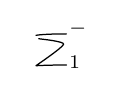
\begin{tikzpicture}[x=0.025em,y=-0.025em,baseline=(base),line cap=round,line join=round]
\coordinate (base) at (0,55);
\path[use as bounding box] (0,0) rectangle (95,65);
\begin{scope}[shift={(-653,-2265)}]
\draw[line width=0.45pt] (665,2276) .. controls (679.1,2274) and (702,2274) .. (709,2274);
\draw[line width=0.45pt] (669,2281) .. controls (677,2282) and (706,2285) .. (705,2289) .. controls (703,2294) and (672,2315) .. (665,2320) .. controls (682.6,2319) and (700,2319) .. (709,2319);
\node[anchor=base west,inner sep=0pt,outer sep=0pt,font=\scriptsize] at (713,2324) {$1$};
\node[anchor=base west,inner sep=0pt,outer sep=0pt,font=\scriptsize] at (713,2274) {$-$};
\node[anchor=base west,inner sep=0pt,outer sep=0pt] at (653,2320) {\phantom{$\Sigma_{1}^{-}$}};
\end{scope}
\end{tikzpicture}
% END C026-S36
\underset{\text{% BEGIN C026-M04
\unsure{\begin{tikzpicture}[x=0.025em,y=-0.025em,baseline=(base),line cap=round,line join=round]
\coordinate (base) at (0,12);
\path[use as bounding box] (0,0) rectangle (12,16);
\begin{scope}[shift={(-749,-2314)}]
\draw[line width=0.35pt,black!60] (754,2318) -- (756,2324);
\end{scope}
\end{tikzpicture}}
% END C026-M04
}}{\cap}% BEGIN C026-S37
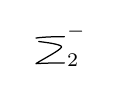
\begin{tikzpicture}[x=0.025em,y=-0.025em,baseline=(base),line cap=round,line join=round]
\coordinate (base) at (0,52);
\path[use as bounding box] (0,0) rectangle (95,63);
\begin{scope}[shift={(-783,-2266)}]
\draw[line width=0.45pt] (795,2281) .. controls (808.1,2279) and (829,2279) .. (836,2279);
\draw[line width=0.45pt] (799,2286) .. controls (807,2287) and (833,2290) .. (832,2294) .. controls (830,2299) and (802,2313) .. (795,2318) .. controls (811.4,2317) and (827,2317) .. (836,2317);
\node[anchor=base west,inner sep=0pt,outer sep=0pt,font=\scriptsize] at (840,2322) {$2$};
\node[anchor=base west,inner sep=0pt,outer sep=0pt,font=\scriptsize] at (840,2279) {$-$};
\node[anchor=base west,inner sep=0pt,outer sep=0pt] at (783,2318) {\phantom{$\Sigma_{2}^{-}$}};
\end{scope}
\end{tikzpicture}
% END C026-S37
\supset E_1\cup E_2,\quad% BEGIN C026-S38
\begin{tikzpicture}[x=0.025em,y=-0.025em,baseline=(base),line cap=round,line join=round]
\coordinate (base) at (0,52);
\path[use as bounding box] (0,0) rectangle (81,62);
\begin{scope}[shift={(-1167,-2257)}]
\draw[line width=0.45pt] (1177,2275) .. controls (1190.8,2273) and (1213,2273) .. (1220,2273);
\draw[line width=0.45pt] (1181,2280) .. controls (1189,2281) and (1217,2284) .. (1216,2288) .. controls (1214,2293) and (1184,2304) .. (1177,2309) .. controls (1194.2,2308) and (1211,2308) .. (1220,2308);
\node[anchor=base west,inner sep=0pt,outer sep=0pt,font=\scriptsize] at (1224,2313) {$1$};
\node[anchor=base west,inner sep=0pt,outer sep=0pt,font=\scriptsize] at (1224,2273) {$-$};
\node[anchor=base west,inner sep=0pt,outer sep=0pt] at (1167,2309) {\phantom{$\Sigma_{1}^{-}$}};
\end{scope}
\end{tikzpicture}
% END C026-S38
\cap% BEGIN C026-S39
\begin{tikzpicture}[x=0.025em,y=-0.025em,baseline=(base),line cap=round,line join=round]
\coordinate (base) at (0,49);
\path[use as bounding box] (0,0) rectangle (86,61);
\begin{scope}[shift={(-1265,-2256)}]
\draw[line width=0.45pt] (1278,2270) .. controls (1291.4,2268) and (1313,2268) .. (1320,2268);
\draw[line width=0.45pt] (1282,2275) .. controls (1290,2276) and (1317,2279) .. (1316,2283) .. controls (1314,2288) and (1285,2300) .. (1278,2305) .. controls (1294.8,2304) and (1311,2304) .. (1320,2304);
\node[anchor=base west,inner sep=0pt,outer sep=0pt,font=\scriptsize] at (1324,2309) {$2$};
\node[anchor=base west,inner sep=0pt,outer sep=0pt,font=\scriptsize] at (1324,2268) {$-$};
\node[anchor=base west,inner sep=0pt,outer sep=0pt] at (1265,2305) {\phantom{$\Sigma_{2}^{-}$}};
\end{scope}
\end{tikzpicture}
% END C026-S39
\ne\varnothing
\end{aligned}
\]
% archive sheet number: 25
